\documentclass[UTF8,a4paper,10pt]{ctexart}
\usepackage[left=2.00cm, right=2.00cm, top=3.50cm, bottom=3.50cm]{geometry} %页边距
\CTEXsetup[format={\Large\bfseries}]{section} %设置章标题居左
 
 
%%%%%%%%%%%%%%%%%%%%%%%
% -- text font --
% compile using Xelatex
%%%%%%%%%%%%%%%%%%%%%%%
% -- 中文字体 --
%\setmainfont{Microsoft YaHei}  % 微软雅黑
%\setmainfont{YouYuan}  % 幼圆    
%\setmainfont{NSimSun}  % 新宋体
%\setmainfont{KaiTi}    % 楷体
%\setmainfont{SimSun}   % 宋体
%\setmainfont{SimHei}   % 黑体
% -- 英文字体 --
%\usepackage{times}
%\usepackage{mathpazo}
%\usepackage{fourier}
%\usepackage{charter}
\usepackage{helvet}
\usepackage{amsmath, amsfonts, amssymb} % math equations, symbols
\usepackage[english]{babel}
\usepackage{color}      % color content
\usepackage{graphicx}   % import figures
\usepackage{url}        % hyperlinks
\usepackage{bm}         % bold type for equations
\usepackage{multirow}
\usepackage{booktabs}
\usepackage{epstopdf}
\usepackage{epsfig}
\usepackage{algorithm}
\usepackage{algorithmic} 
\usepackage{listings} 
\usepackage{xcolor}
\lstset{
    language=matlab,  %代码语言使用的是matlab
    frame=shadowbox, %把代码用带有阴影的框圈起来
    rulesepcolor=\color{red!20!green!20!blue!20},%代码块边框为淡青色
    keywordstyle=\color{blue!90}\bfseries, %代码关键字的颜色为蓝色,粗体
    commentstyle=\color{red!10!green!70}\textit,    % 设置代码注释的颜色
    showstringspaces=false,%不显示代码字符串中间的空格标记
    numbers=left, % 显示行号
    numberstyle=\tiny,    % 行号字体
    stringstyle=\ttfamily, % 代码字符串的特殊格式
    breaklines=true, %对过长的代码自动换行
    extendedchars=false,  %解决代码跨页时,章节标题,页眉等汉字不显示的问题
%   escapebegin=\begin{CJK*},escapeend=\end{CJK*},      
% 代码中出现中文必须加上,否则报错
    texcl=true}
\renewcommand{\algorithmicrequire}{ \textbf{Input:}}     % use Input in the format of Algorithm  
\renewcommand{\algorithmicensure}{ \textbf{Initialize:}} % use Initialize in the format of Algorithm  
\renewcommand{\algorithmicreturn}{ \textbf{Output:}}     % use Output in the format of Algorithm   

% -------------------------允许算法跨页-------------
\makeatletter
\newenvironment{breakablealgorithm}
    {% \begin{breakablealgorithm}
    \begin{center}
        \refstepcounter{algorithm}% New algorithm
        \hrule height.8pt depth0pt \kern2pt% \@fs@pre for \@fs@ruled
        \renewcommand{\caption}[2][\relax]{% Make a new \caption
            {\raggedright\textbf{\ALG@name~\thealgorithm} ##2\par}%
                \ifx\relax##1\relax % #1 is \relax
                    \addcontentsline{loa}{algorithm}{\protect\numberline{\thealgorithm}##2}%
                \else % #1 is not \relax
                    \addcontentsline{loa}{algorithm}{\protect\numberline{\thealgorithm}##1}%
                \fi
            \kern2pt\hrule\kern2pt
        }
  }{% \end{breakablealgorithm}
            \kern2pt\hrule\relax% \@fs@post for \@fs@ruled
        \end{center}
  }
\makeatother
 
\usepackage{fancyhdr} %设置页眉、页脚
%\pagestyle{fancy}
\lhead{}
\chead{}
%\rhead{\includegraphics[width=1.2cm]{fig/ZJU_BLUE.eps}}
\lfoot{}
\cfoot{}
\rfoot{}
%\pagestyle{empty} %删除所有页码
 
%%%%%%%%%%%%%%%%%%%%%%%
%  设置水印
%%%%%%%%%%%%%%%%%%%%%%%
%\usepackage{draftwatermark}         % 所有页加水印
%\usepackage[firstpage]{draftwatermark} % 只有第一页加水印
% \SetWatermarkText{Water-Mark}           % 设置水印内容
% \SetWatermarkText{\includegraphics{fig/ZJDX-WaterMark.eps}}         % 设置水印logo
% \SetWatermarkLightness{0.9}             % 设置水印透明度 0-1
% \SetWatermarkScale{1}                   % 设置水印大小 0-1    
 
\usepackage{hyperref} %bookmarks
\hypersetup{colorlinks, bookmarks, unicode} %unicode
 

\title{\textbf{数值代数第1章上机实验报告}}
\author{ 211840196 张博阳 }
\date{}


\begin{document}
    \maketitle
 
    \section*{摘要}
        \par
        本实验报告基于第1章所学的各解线性方程组的直接法对上机实验题给出了相应的程序实现与执行情况,其中阐述了所使用的各直接法的理论背景和实现以及代码实现上为提升精度和速度所使用的技术,并基于实际程序执行情况反馈对算法的实现结果及其性能进行了评价。无一例外地,直接法在解的数值精度上表现优良,但若不根据矩阵本身的结构特点进行定向优化,其在运算时间上的表现非常糟糕,在面对高阶的线性方程组时几乎束手无策(例如练习6.1.1中$n \ge 100$的情形)。练习6.1.2提供了一种对于直接法解线性方程组可行的算法优化方案,实验结果表明优化结果显著,但算法局限性较大(仅适用于特定结构类型的矩阵)。

    \section{前言}
        \par
        解线性方程组的直接法作为理论代数方法的直接数值化,具有精度高的特点,但自身较高的时间复杂度使得其在面对高阶线性方程组时无法在令人满意的时间内给出计算结果。第1章上机实验题基于直接法的这一特征给出了可利用直接法求解的多个问题及其基于矩阵本身分布特征的改进方法。
 
    \section{数学原理和程序设计流程}
        \subsection{Gauss消去法}
            \par    
            对于待求解线性方程组$Ax=b\ ({\rm rank}\ A=n)$,根据线性代数知识,其与线性方程组$\tilde{A}x=\tilde{b}$同解,其中$[\tilde{A}\ \tilde{b}]$可由$[A\ b]$作有限次初等行变换得到,$\tilde{A}$为上三角矩阵。据${\rm rank}\ A=n$,$\tilde{A}$皆为非零行。消元步骤完成后,执行回代过程解$\tilde{A}x=\tilde{b}$的步骤是显而易见的:只需自角标递减顺序作反解-代入步骤即可得到解向量$x=[x_1\ x_2\ \dots x_n]^{\rm T}$。
            \par
            设$A=(a_{ij})_n\in M^{n\times n}(\mathbb{R}),x=[x_1\ x_2\ \dots x_n]^{\rm T}\in \mathbb{R}^n,b=[b_1\ b_2\ \dots b_n]^{\rm T}\in \mathbb{R}^n$,Gauss消去法的消元过程由$n-1$步组成,记$a_{ij},b_i$在第$k$步消元后得到的元素为$a_{ij}^{(k)},b_i^{(k)}$,规定$a_{ij}^{(0)}=a_{ij},b_i^{(0)}=b_i$。第1步,不妨设$a_{11}\neq0$(否则作适当的行交换),将增广矩阵$[A\ b]$的第1列均消为0:
            $$
            [A^{(1)}\ b^{(1)}]=
                \begin{bmatrix}
                    a_{11}^{(0)} & a_{12}^{(0)} & \cdots & a_{1n}^{(0)} & b_1^{(0)} \\
                    \ & a_{22}^{(1)} & \cdots & a_{2n}^{(1)} & b_2^{(1)} \\
                    \ & \vdots & \ & \vdots & \vdots \\
                    \ & a_{n2}^{(1)} & \cdots & a_{nn}^{(1)} & b_n^{(1)}
                \end{bmatrix}
            $$
            第$k$步,不妨设$a_{kk}^{(k-1)}\neq0$(否则作适当的行交换),将增广矩阵$[A^{(k-1)}\ b^{(k-1)}]$的第$k$列均消为0:
            $$
            [A^{(k)}\ b^{(k)}]=
                \begin{bmatrix}
                    a_{11}^{(0)} & a_{12}^{(0)} & \cdots & a_{1k}^{(0)} & a_{1,k+1}^{(0)} & \cdots & a_{1n}^{(0)} & b_1^{(0)} \\
                    \ & a_{22}^{(1)} & \cdots & a_{2k}^{(1)} & a_{2,k+1}^{(1)} & \cdots & a_{2n}^{(1)} & b_2^{(1)} \\
                    \ & \ & \ddots & \vdots & \vdots & \ & \vdots & \vdots \\
                    \  & \  & \  & a_{kk}^{(k-1)}& a_{k,k+1}^{(k-1)} & \cdots & a_{kn}^{(k-1)} & b_k^{(k-1)} \\
                    \  & \  & \  & \  & a_{k+1,k+1}^{(k)} & \cdots & a_{k+1,n}^{(k)} & b_{k+1}^{(k)} \\
                    \  & \  & \  & \  & \vdots & \  & \vdots & \vdots \\
                    \  & \  & \  & \  & a_{n,k+1}^{(k)} & \cdots & a_{nn}^{(k)} & b_n^{(k)}
                \end{bmatrix}
            $$
            其中对于$i=k+1,\dots,n$
                \begin{align*}
                    & a_{ik}^{(k)}=0 \\
                    & a_{ij}^{(k)}=a_{ij}^{(k-1)}-\frac{a_{ik}^{(k-1)}}{a_{kk}^{(k-1)}}a_{kj}^{(k-1)},j=k+1,\dots,n \\
                    & b_{i}^{(k)}=b_{i}^{(k-1)}-\frac{a_{ik}^{(k-1)}}{a_{kk}^{(k-1)}}b_{k}^{(k-1)}
                \end{align*}
            根据上述过程容易算出消元步骤结束后得到的$\tilde{A}$和$\tilde{b}$:
            $$
            [\tilde{A}\ \tilde{b}]=[A^{(n-1)}\ b^{(n-1)}]
                \begin{bmatrix}
                    a_{11}^{(0)} & a_{12}^{0} & a_{13}^{(0)} & \cdots & a_{1n}^{(0)} & b_1^{(0)} \\
                    \      & a_{22}^{(1)} & a_{23}^{(1)} & \cdots & a_{2n}^{(1)} & b_2^{(1)} \\
                    \ & \ & a_{33}^{(2)} & \cdots & a_{3n}^{(2)} & b_3^{(2)} \\
                    \ & \ & \ & \ddots & \vdots & \vdots \\
                    \ & \ & \ & \ & a_{nn}^{(n-1)} & b_n^{(n-1)}
                \end{bmatrix}
            $$
        \subsection{直接三角分解法}
            \subsubsection{LU分解}
                \par
                根据2.1讨论的Gauss消元法过程可以看出,若系数矩阵$A$的前$n-1$阶顺序主子式$A_1,A_2,\dots,A_{n-1}$皆不为0,则顺序Gauss消元法可以在不进行行交换的情况下进行到底,亦即只需进行前两种初等行变换就可将$[A\ b]$化为$[\tilde{A}\ \tilde{b}]$。注意到对于第$k$次消元操作,对应的行变换矩阵为
                $$
                L_k^{-1}=
                    \begin{bmatrix}
                        1 & \  & \  & \  & \  & \  & \  \\
                        \  & \ddots & \  & \  & \  & \  & \  \\
                        \  & \ & 1 & \  & \  & \  & \  \\
                        \  & \ & \  & 1 & \  & \  & \  \\
                        \  & \ & \  & -\frac{a_{k+1,k}^{(k-1)}}{a_{kk}^{(k-1)}} & 1 & \  & \  \\
                        \  & \ & \  & \vdots & \  & \ddots & \  \\
                        \  & \ & \  & -\dfrac{a_{nk}^{(k-1)}}{a_{kk}^{(k-1)}} & \  & \  & 1
                    \end{bmatrix}
                $$
                从而Gauss消元法有矩阵表示
                    \begin{align*}
                        [\tilde{A}\ \tilde{b}]&=[A^{(n-1)}\ b^{(n-1)}]\\
                        &=[L_{n-1}^{-1}A^{(n-2)}\ L_{n-1}^{-1}b^{(n-2)}]\\
                        &=L_{n-1}^{-1}L_{n-2}^{-1}\dots L_2^{-1}L_1^{-1}[A\ b]
                    \end{align*}
                亦即$A=L_1L_2\dots L_{n-2}L_{n-1}\tilde{A}$。注意到
                $$
                    \begin{bmatrix}
                        1 & \  & \  & \  & \  & \  & \  \\
                        \  & \ddots & \  & \  & \  & \  & \  \\
                        \  & \ & 1 & \  & \  & \  & \  \\
                        \  & \ & \  & 1 & \  & \  & \  \\
                        \  & \ & \  & \dfrac{a_{k+1,k}^{(k-1)}}{a_{kk}^{(k-1)}} & 1 & \  & \  \\
                        \  & \ & \  & \vdots & \  & \ddots & \  \\
                        \  & \ & \  & \dfrac{a_{nk}^{(k-1)}}{a_{kk}^{(k-1)}} & \  & \  & 1
                    \end{bmatrix}
                    \begin{bmatrix}
                        1 & \  & \  & \  & \  & \  & \  \\
                        \  & \ddots & \  & \  & \  & \  & \  \\
                        \  & \ & 1 & \  & \  & \  & \  \\
                        \  & \ & \  & 1 & \  & \  & \  \\
                        \  & \ & \  & -\dfrac{a_{k+1,k}^{(k-1)}}{a_{kk}^{(k-1)}} & 1 & \  & \  \\
                        \  & \ & \  & \vdots & \  & \ddots & \  \\
                        \  & \ & \  & -\dfrac{a_{nk}^{(k-1)}}{a_{kk}^{(k-1)}} & \  & \  & 1
                    \end{bmatrix}=I
                $$
                即
                $$
                L_k=
                    \begin{bmatrix}
                        1 & \  & \  & \  & \  & \  & \  \\
                        \  & \ddots & \  & \  & \  & \  & \  \\
                        \  & \ & 1 & \  & \  & \  & \  \\
                        \  & \ & \  & 1 & \  & \  & \  \\
                        \  & \ & \  & \dfrac{a_{k+1,k}^{(k-1)}}{a_{kk}^{(k-1)}} & 1 & \  & \  \\
                        \  & \ & \  & \vdots & \  & \ddots & \  \\
                        \  & \ & \  & \dfrac{a_{nk}^{(k-1)}}{a_{kk}^{(k-1)}} & \  & \  & 1
                    \end{bmatrix}
                $$
                且诸$L_k$皆为下三角阵,从而$L=L_1L_2\dots L_{n-2}L_{n-1}$也为下三角阵。又$\tilde{A}$为上三角阵,记$U=\tilde{A}$,则$A$可分解为$A=LU$的形式,进而解线性方程组$Ax=b$问题转化为解两个系数矩阵为上(下)三角矩阵的线性方程组$Ly=b,Ux=y$。
                \par
                直接计算可以得到$L$和$U$:
                $$
                L=
                    \begin{bmatrix}
                        1 & \  & \  & \  & \  & \  \\
                        \dfrac{a_{21}^{(0)}}{a_{11}^{(0)}} & 1 & \  & \  & \  & \  \\
                        \dfrac{a_{31}^{(0)}}{a_{11}^{(0)}} & \dfrac{a_{32}^{(1)}}{a_{22}^{(1)}} & 1 & \  & \  & \  \\
                        \vdots & \vdots & \ddots  & \ddots & \ \\
                        \dfrac{a_{n-1,1}^{(0)}}{a_{11}^{(0)}} & \dfrac{a_{n-1,2}^{(1)}}{a_{22}^{(1)}} & \cdots & \dfrac{a_{n-1,n-2}^{(n-3)}}{a_{n-2,n-2}^{(n-3)}} & 1 \\
                        \dfrac{a_{n1}^{(0)}}{a_{11}^{(0)}} & \dfrac{a_{n2}^{(1)}}{a_{22}^{(1)}} & \cdots & \dfrac{a_{n,n-2}^{(n-3)}}{a_{n-2,n-2}^{(n-3)}} & \dfrac{a_{n,n-1}^{(n-2)}}{a_{n-1,n-1}^{(n-2)}} & 1 \\
                    \end{bmatrix}
                $$
                $$
                U=
                    \begin{bmatrix}
                        a_{11}^{(0)} & a_{12}^{(0)} & a_{13}^{(0)} & \cdots & a_{1n}^{(0)} \\
                        \ & a_{22}^{(1)} & a_{23}^{(1)} & \cdots & a_{2n}^{(1)} \\
                        \ & \ & a_{33}^{(2)} & \cdots & a_{3n}^{(2)} \\
                        \ & \ & \ & \ddots & \vdots \\
                        \ & \ & \ & \ & a_{nn}^{(n-1)}
                    \end{bmatrix}
                $$
                此处$L$为单位下三角阵,亦即给出了对系数矩阵$A$的Doolittle分解。注意到
                    \begin{align*}
                        LU&=
                        \begin{bmatrix}
                            1 & \  & \  & \  & \  & \  \\
                            \dfrac{a_{21}^{(0)}}{a_{11}^{(0)}} & 1 & \  & \  & \  & \  \\
                            \dfrac{a_{31}^{(0)}}{a_{11}^{(0)}} & \dfrac{a_{32}^{(1)}}{a_{22}^{(1)}} & 1 & \  & \  & \  \\
                            \vdots & \vdots & \ddots  & \ddots & \ \\
                            \dfrac{a_{n-1,1}^{(0)}}{a_{11}^{(0)}} & \dfrac{a_{n-1,2}^{(1)}}{a_{22}^{(1)}} & \cdots & \dfrac{a_{n-1,n-2}^{(n-3)}}{a_{n-2,n-2}^{(n-3)}} & 1 \\
                            \dfrac{a_{n1}^{(0)}}{a_{11}^{(0)}} & \dfrac{a_{n2}^{(1)}}{a_{22}^{(1)}} & \cdots & \dfrac{a_{n,n-2}^{(n-3)}}{a_{n-2,n-2}^{(n-3)}} & \dfrac{a_{n,n-1}^{(n-2)}}{a_{n-1,n-1}^{(n-2)}} & 1 \\
                        \end{bmatrix}
                        \begin{bmatrix}
                            a_{11}^{(0)} & a_{12}^{(0)} & a_{13}^{(0)} & \cdots & a_{1n}^{(0)} \\
                            \ & a_{22}^{(1)} & a_{23}^{(1)} & \cdots & a_{2n}^{(1)} \\
                            \ & \ & a_{33}^{(2)} & \cdots & a_{3n}^{(2)} \\
                            \ & \ & \ & \ddots & \vdots \\
                            \ & \ & \ & \ & a_{nn}^{(n-1)}
                        \end{bmatrix}\\
                        &=
                        \begin{bmatrix}
                            1 & \  & \  & \  & \  & \  \\
                            \dfrac{a_{21}^{(0)}}{a_{11}^{(0)}} & 1 & \  & \  & \  & \  \\
                            \dfrac{a_{31}^{(0)}}{a_{11}^{(0)}} & \dfrac{a_{32}^{(1)}}{a_{22}^{(1)}} & 1 & \  & \  & \  \\
                            \vdots & \vdots & \vdots  & \ddots & \ \\
                            \dfrac{a_{n1}^{(0)}}{a_{11}^{(0)}} & \dfrac{a_{n2}^{(1)}}{a_{22}^{(1)}} & \dfrac{a_{n,3}^{(2)}}{a_{3,3}^{(2)}} & \cdots & 1 \\
                        \end{bmatrix}
                        \begin{bmatrix}
                            a_{11}^{(0)} & \  & \  & \  &  \  \\
                            \  & a_{22}^{(1)}  & \  & \  &  \  \\
                            \  & \  & a_{33}^{(2)} & \  &  \  \\
                            \  & \  & \  & \ddots & \ \\
                            \  & \  & \  & \  & a_{nn}^{(n-1)} \\
                        \end{bmatrix}
                        \begin{bmatrix}
                            1 & \dfrac{a_{12}^{(0)}}{a_{22}^{(1)}} & \dfrac{a_{13}^{(0)}}{a_{33}^{(2)}} & \cdots & \dfrac{a_{1n}^{(0)}}{a_{nn}^{(n-1)}} \\
                            \ & 1 & \dfrac{a_{23}^{(1)}}{a_{33}^{(2)}} & \cdots & \dfrac{a_{2n}^{(1)}}{a_{nn}^{(n-1)}} \\
                            \ & \ & 1 & \cdots & \dfrac{a_{3n}^{(2)}}{a_{nn}^{(n-1)}} \\
                            \ & \ & \ & \ddots & \vdots \\
                            \ & \ & \ & \ & 1
                        \end{bmatrix}
                        =\tilde{L}D\tilde{U}\\
                        &=
                        \begin{bmatrix}
                            a_{11}^{(0)} & \  & \  & \  & \  & \  \\
                            a_{21}^{(0)} & a_{22}^{(1)} & \  & \  & \  & \  \\
                            a_{31}^{(0)} & a_{32}^{(1)} & a_{33}^{(2)} & \  & \  & \  \\
                            \vdots & \vdots & \vdots  & \ddots & \ \\
                            a_{n1}^{(0)} & a_{n2}^{(1)} & a_{n3}^{(2)} & \cdots & a_{nn}^{(n-1)} \\
                        \end{bmatrix}
                        \begin{bmatrix}
                            1 & \dfrac{a_{12}^{(0)}}{a_{22}^{(1)}} & \dfrac{a_{13}^{(0)}}{a_{33}^{(2)}} & \cdots & \dfrac{a_{1n}^{(0)}}{a_{nn}^{(n-1)}} \\
                            \ & 1 & \dfrac{a_{23}^{(1)}}{a_{33}^{(2)}} & \cdots & \dfrac{a_{2n}^{(1)}}{a_{nn}^{(n-1)}} \\
                            \ & \ & 1 & \cdots & \dfrac{a_{3n}^{(2)}}{a_{nn}^{(n-1)}} \\
                            \ & \ & \ & \ddots & \vdots \\
                            \ & \ & \ & \ & 1
                        \end{bmatrix}
                        =L'U'
                    \end{align*}
                这就给出了对系数矩阵$A$的$LDU$分解和Crout分解。可以证明,当$A$的顺序主子阵$A_1,A_2,\dots,A_{n-1}$皆非奇异(即顺序Gauss消元法可以执行到底)时,$LDU$分解是唯一的。
            \subsubsection{Cholesky分解}
                \par
                对于实对称正定的系数矩阵$A$,有更好的结果Cholesky分解在,即存在下三角阵$L$使得$A=LL^{\rm T}$。设$L=(l_{ij})_n,l_{ij}=0(i<j)$。直接计算可得
                $$
                    \begin{cases}
                        \sum_{k=1}^jl_{ik}l_{jk}=a_{ij}, & i>j \\
                        \sum_{k=1}^il_{ik}^2=a_{ii}, & i=j
                    \end{cases}
                $$
                逐步回代反解即得$L$各元素计算式
                $$
                l_{lj}=
                    \begin{cases}
                        \sqrt{a_{ii}-\sum_{k=1}^{i-1}l_{ik}^2}, & i=j \\
                        \dfrac{a_{ij}-\sum_{k=1}^{j-1}l_{ik}l_{jk}}{l_{jj}}, & i>j \\
                        0, & i<j
                    \end{cases}
                $$
                和$LU$分解的情形类似,可以作出实对称正定矩阵$A$的$LDL^{\rm T}$分解。记$D={\rm diag}(d_1,d_2,\dots,d_n),d_{ii}>0$,则
                $$
                l_{lj}=
                    \begin{cases}
                        1, & i=j \\
                        \dfrac{a_{ij}-\sum_{k=1}^{j-1}l_{ik}d_kl_{jk}}{d_{j}}, & i>j \\
                        0, & i<j
                    \end{cases}
                $$
                $$
                d_i=a_{ii}-\sum_{k=1}^{i-1}l_{ik}d_kl_{ik},i=1,2,\dots,n
                $$
            \subsubsection{基于Crout分解的解三对角线性方程组的追赶法}
                \par
                考虑三对角线性方程粗$Ax=b$,其中
                $$
                A=
                    \begin{bmatrix}
                        d_1 & c_1 & \  & \  & \  & \  \\
                        a_2 & d_2 & c_2 & \  & \  & \  \\
                        \  & a_3 & d_3 & c_3 & \  & \  \\
                        \  & \  & \ddots & \ddots & \ddots & \  \\
                        \  & \  & \  & a_{n-1} & d_{n-1} & c_{n-1} \\
                        \  & \  & \  & \  & a_n & d_n
                    \end{bmatrix}
                $$
                由于三对角矩阵$A$稀疏程度高,直接使用Gauss消元法会导致大量冗余计算步骤,计算效率降低。考虑对$A$作Crout分解
                $$
                A=LU=
                    \begin{bmatrix}
                        p_1 & \  & \  & \  \\
                        a_2 & p_2 & \  & \  & \  \\
                        \  & a_3 & p_3 & \  & \  \\
                        \  & \  & \ddots & \ddots & \  \\
                        \  & \  & \  & a_n & p_n
                    \end{bmatrix}
                    \begin{bmatrix}
                        1 & q_1  & \  & \  \\
                        \  & 1 & q_2  & \  & \  \\
                        \  & \  & 1 & q_3  & \  \\
                        \  & \  & \  & \ddots & \ddots & \  \\
                        \  & \  & \  & \  & \ddots & q_{n-1} \\
                        \  & \  & \  & \  & \  & 1
                    \end{bmatrix}
                $$
                根据Crout分解计算公式,容易化简出上述两矩阵各元素的计算式:
                $$
                p_k=
                    \begin{cases}
                        d_1,&k=1 \\
                        d_k-a_kq_{k-1},&k=2,\dots,n
                    \end{cases}
                $$
                $$
                q_k=
                    \begin{cases}
                        \dfrac{c_1}{d_1},&k=1 \\
                        \dfrac{c_k}{p_k},&k=2,\dots,n
                    \end{cases}
                $$
                进而可以将解线性方程组$Ax=b$的问题转化为$Ly=b$和$Ux=y$。可以算得
                $$
                y_k=
                    \begin{cases}
                        \dfrac{b_1}{d_1},&k=1 \\
                        \dfrac{b_k-a_ky_{k-1}}{p_k},&k=2,\dots,n
                    \end{cases}
                $$
                $$
                x_k=
                    \begin{cases}
                        y_k-q_kx_{k+1},&k=1,\dots,n-1 \\
                        y_k,&k=n
                    \end{cases}
                $$
        \subsection{基于Gauss-Jordan消去法的逆矩阵算法}
            Gauss消元法通过初等行变换将主对角线下方的各元素消为0,对称地,可以采用同样方法把主对角线上方的各元素也消为0,亦即将系数矩阵变为对角阵。进一步地,如果再作主对角线元素除以自身的操作,即可将系数矩阵化为单位阵。上述过程用矩阵表述为
            $$
            A^{(k)}=M_kA^{(k-1)}
            $$
            其中
            $$
            M_k=
                \begin{bmatrix}
                    1 & \  & \  & m_{1k} & \  & \  & \  \\
                    \  & \ddots & \  & \vdots & \  & \  & \  \\
                    \  & \  & 1 & m_{k-1,k} & \  & \  & \  \\
                    \  & \  & \  & m_{kk} & \  & \  & \  \\
                    \  & \  & \  & m_{k+1,k} & 1 & \  & \  \\
                    \  & \  & \  & \vdots & \  & \ddots & \  \\
                    \  & \  & \  & m_{nk} & \  & \  & 1
                \end{bmatrix}
            $$
            $$
            m_{ik}=
                \begin{cases}
                    \dfrac{1}{a_{kk}^{(k-1)}},&i=k, \\
                    -\dfrac{a_{ik}^{(k-1)}}{a_{kk}^{(k-1)}},&i\neq k,
                \end{cases}
            \ \ i=1,2,\dots,n
            $$
            故一方面
            $$
            M_n M_{n-1} \dots M_2 M_1 A=A^{(n)}=I
            $$
            另一方面,$A$的逆满足$XA=I$,并且满足方程的矩阵是唯一的,从而$A$可逆且
            $$
            A^{-1}=M_n M_{n-1} \dots M_2 M_1
            $$
        \subsection{针对问题的程序设计流程}
            \subsubsection{练习6.1.1}
                \par
                首先给出基于上述数学原理的列主元Gauss消去法、对称正定矩阵的$LL^{\rm T}$分解法和$LDL^{\rm T}$分解法的算法流程和伪代码。
                \renewcommand{\thealgorithm}{1}
                \begin{breakablealgorithm}
                        \caption{列主元Gauss消去法}
                        \begin{algorithmic}[1]
                            \REQUIRE $n$阶系数矩阵$A=[\alpha_1^{(0)},\alpha_2^{(0)},\dots,\alpha_n^{(0)}]^{\rm T}=(a_{ij})_n$,右端向量$b=[b_1,b_2,\dots,b_n]^{\rm T}$
                            \FOR {$i=1,\dots,n$}
                                \STATE $p\leftarrow\arg \max_{1 \le p \le n} \left| a_{pi}\right|$ \\
                                \STATE $\alpha_p^{(i-1)}$与$\alpha_i^{(i-1)}$交换 \\
                                \FOR {$j=i+1,\dots,n$}
                                    \FOR {$k=i,\dots,n$}
                                        \STATE $a_{jk}\leftarrow a_{jk}-\dfrac{a_{ii}}{a_{ji}}a_{ik}$ \\
                                    \ENDFOR
                                    \STATE $b_j \leftarrow b_j-\dfrac{a_{ii}}{a_{ji}}b_i$ \\
                                \ENDFOR
                            \ENDFOR
                            \FOR {$i=n,n-1,\dots,1$}
                                \STATE $x_i \leftarrow \dfrac{b_i-\sum_{j=i+1}^{n}a_{ij}x_j}{a_{ii}}$ \\
                            \ENDFOR
                            \RETURN 线性方程组$Ax=b$的解向量$x=[x_1,x_2,\dots,x_n]^{\rm T}$
                        \end{algorithmic}
                    \end{breakablealgorithm}
                    \renewcommand{\thealgorithm}{2}
                    \begin{breakablealgorithm}
                        \caption{对称正定矩阵的$LL^{\rm T}$分解法}
                        \begin{algorithmic}[1]
                            \REQUIRE $n$阶对称正定系数矩阵$A=(a_{ij})_n$,右端向量$b=[b_1,b_2,\dots,b_n]^{\rm T}$
                            \FOR {$i=1,\dots,n$}
                                \STATE $a_{ii} \leftarrow \sqrt{a_{ii}-\sum_{j=1}^{i-1}a_{ij}^2}$ \\
                                \FOR {$j=1,\dots,i-1$}
                                    \STATE $a_{ji} \leftarrow 0$ \\
                                \ENDFOR
                                \FOR {$j=i+1,\dots,n$}
                                    \STATE $a_{ji} \leftarrow \dfrac{a_{ji}-\sum_{k=1}^{i-1}a_{jk}a_{ik}}{a_{ii}}$ \\
                                \ENDFOR
                            \ENDFOR
                            \FOR {$i=1,\dots,n$}
                                \STATE $x_i \leftarrow \dfrac{b_i-\sum_{j=1}^{i-1}a_{ij}x_j}{a_{ii}}$ \\
                            \ENDFOR
                            \FOR {$i=n,n-1,\dots,1$}
                                \STATE $x_i \leftarrow \dfrac{x_i-\sum_{j=i+1}^{n}a_{ji}x_j}{a_{ii}}$ \\
                            \ENDFOR
                            \RETURN 线性方程组$Ax=b$的解向量$x=[x_1,x_2,\dots,x_n]^{\rm T}$
                        \end{algorithmic}
                    \end{breakablealgorithm}
                \par
                在实现$LDL^{\rm T}$方法时,基于减少乘除运算的考虑,取$G=(g_{ij})_n$,其中$g_{ij}=l_{ji}d_i$,则$G$为上三角矩阵。计算可知
                $$
                d_k=
                    \begin{cases}
                        a_{11},&k=1\\
                        a_{kk}-\sum_{j=1}^{i-1}g_{ki}l_{ik},&k=2,\dots,n\\
                    \end{cases}
                $$
                $$
                g_{ij}=
                    \begin{cases}
                        a_{11},&i=1\\
                        a_{ji}-\sum_{k=1}^{j-1}g_{ik}l_{kj}\ (j=1,\dots,i-1),&i=2,\dots,n\\
                    \end{cases}
                $$
                $$
                l_{ij}=\dfrac{g_{ji}}{d_j}\ (j=1,\dots,i-1)
                $$
                    \renewcommand{\thealgorithm}{3}
                    \begin{breakablealgorithm}
                        \caption{对称正定矩阵的$LDL^{\rm T}$分解法}
                        \begin{algorithmic}[1]
                            \REQUIRE $n$阶对称正定系数矩阵$A=(a_{ij})_n$,右端向量$b=[b_1,b_2,\dots,b_n]^{\rm T}$
                            \FOR {$i=1,\dots,n$}
                                \FOR {$j=1,\dots,i-1$}
                                    \STATE $a_{ji} \leftarrow a_{ij}-\sum_{k=1}^{j-1}a_{jk}a_{ki}$ \\
                                    \STATE $a_{ij} \leftarrow \dfrac{a_{ji}}{a_{jj}}$ \\
                                \ENDFOR
                                \STATE $a_{ii} \leftarrow a_{ii}-\sum_{j=1}^{i-1}a_{ij}a_{ji}$ \\
                            \ENDFOR
                            \FOR {$i=1,\dots,n$}
                                \STATE $x_i \leftarrow b_i-\sum_{j=1}^{i-1}a_{ij}x_j$ \\
                            \ENDFOR
                            \FOR {$i=n,n-1,\dots,1$}
                                \STATE $x_i \leftarrow \dfrac{x_i}{a_{ii}}-\sum_{j=i+1}^{n}a_{ji}x_j$ \\
                            \ENDFOR
                            \RETURN 线性方程组$Ax=b$的解向量$x=[x_1,x_2,\dots,x_n]^{\rm T}$
                        \end{algorithmic}
                    \end{breakablealgorithm}
                \par
                就练习6.1.1编写的Matlab程序整体上遵循面向过程的编程思想,主程序存放在脚本\texttt{work\_611.m}中;用脚本文件\texttt{Maximal\_Column\_Pivoting\_Gauss.m}、\texttt{LLT.m}、\texttt{LDLT.m}分别封装函数\texttt{Maximal\_Column\_Pivoting\_Gauss}、\texttt{LLT}、\texttt{LDLT},其输入参数列表为系数矩阵A,输出分别对A用列主元Gauss消元法、$LL^{\rm T}$分解、$LDL^{\rm T}$分解解线性方程组$Ax=b$所得解向量$x$;脚本文件\texttt{algorithm\_error.m}、\texttt{algorithm\_time.m}和\texttt{matrix\_condition.m}分别封装数值误差(对数坐标)、CPU运行时间和矩阵条件数关于参量$n$的绘图函数。程序以矩阵和向量为基本操作对象,其代码属于BLAS-2代码,具有较好的可读性。
                \par
                在算法具体实现上,由于函数参数列表采用值传递方式,输入参数在函数中存在副本,因此考虑将计算所得结果尽可能覆盖参数副本存储空间,以使存储空间得到充分利用。脚本\texttt{LLT.m}、\texttt{LDLT.m}充分利用了数据覆盖技术,最大限度地使用了存储空间。\texttt{LLT.m}在三角分解结束后用$L$覆盖了$A$,\texttt{LDLT.m}在三角分解结束后利用$L$为单位下三角阵,$D,G$有相同的主对角元素的结构特点,用$L,D,G$覆盖了$A$。两脚本中间变量$y=[y_1,y_2,\dots,y_n]^{\rm T}$与解向量$x=[x_1,x_2,\dots,x_n]^{\rm T}$皆共用同一$n$维数组存储空间。
            \subsubsection{练习6.1.2}
                \par
                一般Crout算法(即固定$U$的对角元为1的$LU$分解)的算法流程与伪代码如下:
                    \renewcommand{\thealgorithm}{4.1}
                    \begin{breakablealgorithm}
                        \caption{一般Crout算法}
                        \begin{algorithmic}[1]
                            \REQUIRE $n$阶矩阵$A$,其中顺序主子阵$A_1,A_2,\dots,A_{n-1}$皆非奇异
                            \FOR {$i=1,\dots,n$}
                                \FOR {$j=i,i+1,\dots,n$}
                                    \STATE $a_{ji} \leftarrow a_{ji}-\sum_{k=1}^{i-1}a_{jk}a_{ki}$ \\
                                \ENDFOR
                                \FOR {$j=i+1,\dots,n$}
                                    \STATE $a_{ij} \leftarrow \dfrac{a_{ij}-\sum_{k=1}^{i-1}a_{ik}a_{kj}}{a_{ii}}$ \\
                                \ENDFOR
                            \ENDFOR
                            \RETURN 计算后的矩阵$A$,其中主对角线及下方元素组成矩阵$L$,主对角线上方元素组成$U$的非对角元,$U$的对角元默认为1
                        \end{algorithmic}
                    \end{breakablealgorithm}
                此处亦使用了数据覆盖技术。
                \par
                易见问题所研究的矩阵$\mathbb{B}_1$和$\mathbb{B}_2$在$n$充分大时稀疏程度均较高,就$\mathbb{B}_1$和$\mathbb{B}_2$各自的元素分布特点,对一般的Crout算法进行了改进,用赋值操作替换不必要的计算步骤以提升计算效率。
                \par
                对于$\mathbb{B}_1$,注意到作$LU$分解后所得矩阵仅在$(n,n)$元素位置与原矩阵有差异,归纳可证对于$\mathbb{B}_1=(b_{ij}^{(1)})_n$及对应$LU$分解所得矩阵$\tilde{\mathbb{B}}_1=(\tilde{b}_{ij}^{(1)})_n$,有
                $$
                b_{ij}^{(1)}=\tilde{b}_{ij}^{(1)}
                $$
                其中$i,j$满足
                $$
                \delta_{in}\delta_{jn}\neq1
                $$
                直接计算可知
                $$
                \tilde{b}_{nn}^{(1)}=b_{nn}^{(1)}-\sum_{i=1}^{n-1}\tilde{b}_{ni}^{(1)}\tilde{b}_{in}^{(1)}=b_{nn}^{(1)}-\sum_{i=1}^{n-1}b_{ni}^{(1)}b_{in}^{(1)}
                $$
                据此可针对$\mathbb{B}_1$型矩阵修改算法,见Algorithm 4.2。
                    \renewcommand{\thealgorithm}{4.2}
                    \begin{breakablealgorithm}
                        \caption{针对$n$阶$\mathbb{B}_1$型矩阵的改进Crout算法}
                        \begin{algorithmic}[1]
                            \REQUIRE 形如$\mathbb{B}_1$的$n$阶矩阵$A$
                            \STATE $a_{nn} \leftarrow a_{nn}-\sum_{i=1}^{n-1}a_{ni}a_{in}$ \\
                            \RETURN 计算后的矩阵$A$,其中主对角线及下方元素组成矩阵$L$,主对角线上方元素组成$U$的非对角元,$U$的对角元默认为1
                        \end{algorithmic}
                    \end{breakablealgorithm}
                \par
                对于$\mathbb{B}_2$,与$\mathbb{B}_1$情形类似,归纳可证对于$\mathbb{B}_2=(b_{ij}^{(2)})_n$及对应$LU$分解所得矩阵$\tilde{\mathbb{B}}_2=(\tilde{b}_{ij}^{(2)})_n$
                $$
                \tilde{b}_{21}^{(2)}=b_{21}^{(2)},\tilde{b}_{12}^{(2)}=b_{12}^{(2)},i=1,\dots,n
                $$
                $$
                \tilde{b}_{ij}^{(2)}=\tilde{b}_{i,i+1}^{(2)},j=i+1,\dots,n
                $$
                $$
                \tilde{b}_{ij}^{(2)}=\tilde{b}_{j+1,j}^{(2)},i=j+1,\dots,n
                $$
                亦即只需算$\tilde{\mathbb{B}}_2$主对角线及两侧对角线上的元素。进一步地,可以证明当$n \ge 4$时两侧对角线元素有
                $$
                \tilde{b}_{i,i+1}=\tilde{b}_{i-2,i+1},i=3,\dots,n
                $$
                故进一步简化为算$\tilde{\mathbb{B}}_2$的主对角线、主对角线上侧对角线元素及$\tilde{b}_{32}^{(2)}$元,共$2n$个元素,据此针对$\mathbb{B}_2$型矩阵修改算法,见Algorithm 4.3。
                    \renewcommand{\thealgorithm}{4.3}
                    \begin{breakablealgorithm}
                        \caption{针对$n$阶$\mathbb{B}_2$型矩阵的改进Crout算法}
                        \begin{algorithmic}[1]
                            \REQUIRE 形如$\mathbb{B}_2$的$n$阶矩阵$A,n \ge 4$
                            \STATE $a_{22} \leftarrow a_{22}-a_{21}a_{12}$ \\
                            \STATE $a_{32} \leftarrow a_{32}-a_{31}a_{13}$ \\
                            \STATE $a_{23} \leftarrow \dfrac{a_{23}-a_{21}a_{13}}{a_{22}}$ \\
                            \FOR {$j=4,\dots,n$}
                                    \STATE $a_{j2} \leftarrow a_{32}$ \\
                                    \STATE $a_{2j} \leftarrow a_{23}$ \\
                                    \ENDFOR
                            \FOR {$i=3,\dots,n-1$}
                                \STATE $a_{ii} \leftarrow a_{ii}-\sum_{j=1}^{i-1}a_{ij}a_{ji}$ \\
                                \STATE $a_{i+1,i} \leftarrow a_{i-1,i}$ \\
                                \STATE $a_{i,i+1} \leftarrow \dfrac{a_{i,i+1}-\sum_{j=1}^{i-1}a_{ij}a_{j,i+1}}{a_{ii}}$ \\
                                    \FOR {$j=i+2,\dots,n$}
                                        \STATE $a_{ji} \leftarrow a_{i+1,i}$ \\
                                        \STATE $a_{ij} \leftarrow a_{i,i+1}$ \\
                                    \ENDFOR
                            \ENDFOR
                            \STATE $a_{nn} \leftarrow a_{nn}-\sum_{j=1}^{n-1}a_{ni}a_{in}$ \\
                            \RETURN 计算后的矩阵$A$,其中主对角线及下方元素组成矩阵$L$,主对角线上方元素组成$U$的非对角元,$U$的对角元默认为1
                        \end{algorithmic}
                    \end{breakablealgorithm}
            \subsubsection{练习6.1.3}
                \par
                基于Gauss-Jordan消去法的逆矩阵算法流程及伪代码如下:
                    \renewcommand{\thealgorithm}{5}
                    \begin{breakablealgorithm}
                        \caption{使用Gauss-Jordan消去法计算矩阵的逆}
                        \begin{algorithmic}[1]
                            \REQUIRE $n$阶三对角阵$T=(t_{ij})_n$
                            \FOR {$k=1,\dots,n$}
                                \STATE $t_{kk} \leftarrow \dfrac{1}{t_{kk}}$ \\
                                \STATE $t_{ik} \leftarrow -t_{ik}t_{kk},i=1,\dots,n,i \neq k$ \\
                                \STATE $t_{ij} \leftarrow t_{ij}+t_{ik}t_{kj},i=1,\dots,n,j=1,\dots,n,i \neq k,j \neq k$ \\
                                \STATE $t_{kj} \leftarrow t_{kj}t_{kk},j=1,\dots,n,j \neq k$ \\
                            \ENDFOR
                            \RETURN 矩阵$T$的逆$T^{-1}$
                        \end{algorithmic}
                    \end{breakablealgorithm}
                利用数据覆盖技术,逆矩阵$T^{-1}$存放在原矩阵$T$的存储空间内。
            \subsubsection{练习6.1.4}
                \par
                系数矩阵为三对角矩阵的线性方程组追赶法求解的算法流程和伪代码如下:
                    \renewcommand{\thealgorithm}{6}    
                    \begin{breakablealgorithm}
                        \caption{追赶法求解线性方程组}
                        \begin{algorithmic}[1]
                            \REQUIRE $n$阶三对角矩阵$A=(a_{ij})_n$,右端向量$b=[b_1,b_2,\dots,b_n]^{\rm T}$
                            \STATE $a_{12} \leftarrow \dfrac{a_{12}}{a_{11}}$ \\
                            \FOR {$i=2,\dots,n-1$}
                                \STATE $a_{ii} \leftarrow a_{ii}-a_{i,i-1}a_{i-1,i}$ \\
                                \STATE $a_{i,i+1} \leftarrow \dfrac{a_{i,i+1}}{a_{ii}}$ \\
                            \ENDFOR
                            \STATE $a_{nn} \leftarrow a_{nn}-a_{n,n-1}a_{n-1,n}$ \\
                            \STATE $x_1 \leftarrow \dfrac{b_1}{a_{11}}$ \\
                            \FOR {$i=2,\dots,n$}
                                \STATE $x_i \leftarrow \dfrac{b_i-a_{i,i-1}x_{i-1}}{a_{ii}}$ \\
                            \ENDFOR
                            \FOR {$i=n-1,n-2,\dots,1$}
                                \STATE $x_i \leftarrow x_i-a_{i,i+1}x_{i+1}$ \\
                            \ENDFOR
                            \RETURN 线性方程组$Ax=b$的解向量$x$
                        \end{algorithmic}
                    \end{breakablealgorithm}
                中间变量$y=[y_1,y_2,\dots,y_n]^{\rm T}$与解向量$x=[x_1,x_2,\dots,x_n]^{\rm T}$共用同一$n$维数组存储空间,$x$按角标对应覆盖$y$的各元素。

\section{实验结果和数据讨论}
    \subsection{练习6.1.1}
        \par
        主程序\texttt{work\_611.m}的运行结果如Figure 1-4所示。
        \par
        数值误差上,相对而言总体上$LDL^{\rm T}$算法数值误差最小,$LL^{\rm T}$其次,列主元Gauss消去法误差最大,亦即即使Gauss消去法利用列主元方法降低数值误差,其效果依然不如依据系数矩阵本身信息直接进行分解;就本身数值误差绝对值而言,三者在$n=50$(即2500阶线性方程组)误差均在$10^{-12}$数量级以下,获得了精度上令人满意的数值解。
        \par
        CPU运行时间上,相对而言总体上$LDL^{\rm T}$算法运行时间亦最短,$LL^{\rm T}$其次,列主元Gauss消去法时间最长。值得指出的是,在程序实现时为降低运行时间,已将行交换优化为指标向量内元素交换,亦即实现了系数矩阵行间的逻辑交换,但其效果不如依据系数矩阵本身信息直接进行分解;在实际运行时间上,$n$在40-50范围内时解单个线性方程组三种方法所需运行时间皆超过1秒,列主元Gauss消去法已经花费接近30秒来解单个线性方程组,在运行时间上不能很好的满足需求。
        \par
        综合来看,$LDL^{\rm T}$算法在数值误差和CPU计算时间上皆具有优势,$LL^{\rm T}$其次,列主元Gauss消去法表现最差。
        \par
        Figure 3给出了矩阵$\mathbb{A}_{n^2}$的条件数$\kappa_\infty(\mathbb{A}_{n^2})$随$n$的增长。由于$\left\| \mathbb{A}_{n^2} \right\|_\infty$为定值,因此$\kappa_\infty(\mathbb{A}_{n^2})$与$\left\| \mathbb{A}_{n^2}^{-1} \right\|_\infty$成正比,随$n$以多项式速度快速增长(六次以下多项式拟合结果残差范数和皆在4以下)。
        \par
        为验证(1.4.26)式对于相对误差的估计准确性,只需验证
        $$
        f(n)=\dfrac{\left\| \delta x \right\|_\infty}{\left\| x \right\|_\infty n^3 \theta \eta(\mathbb{A}_{n^2})\kappa_\infty(\mathbb{A}_{n^2})}
        $$
        对于某个与$n$无关的常数$C$一致有界,亦即$\left|f(n)\right|\le C$对一切$n$皆成立。$f(n)$关于$n$的图像如Figure 4所示,易见$\left|f(n)\right|\le 1$,满足(1.4.26)式的相对误差估计。
    \subsection{练习6.1.2}
        \par
        程序的执行结果如Figure 5-9所示,其中Figure 7-9给出了$11\le n\le 500$的图像,参数$a=3$。
        \par
        从Figure 5,6中看到,$\mathbb{B}_1$在$LU$分解后稀疏程度保持不变,而$\mathbb{B}_2$计算后变为稠密矩阵。
        \par
        Figure 7中,由于Crout算法的时间复杂度为$O(n^3)$,一般Crout算法并未利用矩阵的特殊结构降低计算量,二者计算时间基本相同,三次函数拟合结果$R^2=0.9982$,符合理论分析结果。
        \par
        改进后$\mathbb{B}_1$的Crout算法时间复杂度降为$O(n)$,$\mathbb{B}_2$的Crout算法时间复杂度为$O(n^2)$。Figure 8、9的结果表明改进效果显著,计算时间大幅下降;$\mathbb{B}_2$的Crout算法时间复杂度关于$n$的二次函数拟合结果$R^2=0.9667$,符合理论结果。
    \subsection{练习6.1.3}
        \par
        程序的执行结果如Figure 10所示,其中$n\le 1000$的图像。
        \par
        根据2.3节对Gauss-Jordan算法的分析,其时间复杂度为$O(n^3)$,图像用三次函数拟合所得$R^2=0.9957$,符合理论结果。

    \subsection{练习6.1.4}
        \par
        程序的执行结果如Figure 11所示,两线性方程组数值误差相同,且问题均具有很好的数值稳定性,但数值误差在总体趋势上并不是单调的。在$n=200,600$时分别出现了局部最低点,在$800<n<1400$范围内数值误差反而随$n$的增长而逐渐下降。

\section{小结}
    \par
    通过上述实验题,解线性方程组的直接法的优势和劣势均被充分地展现出来:所算得的数值解的极高精度(如果能算出来)及其随阶数上升而快速上涨的计算时间,其基于结构的优化算法泛用性也较低。这迫使寻找其他的解线性方程组计算方法,即牺牲一定的精度换取计算时间的下降和算法泛用性的提升。
    
\begin{figure*}[ht]
    \centering
    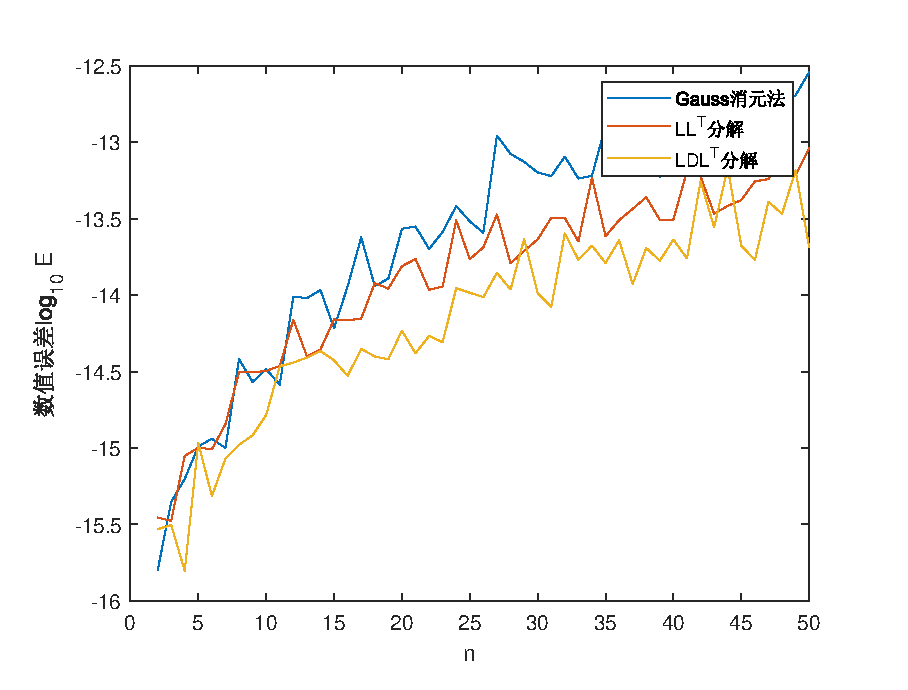
\includegraphics[width=14cm,height=10cm]{1.1_error.eps}
    \caption{The numerical error of three direct methods}
\end{figure*}
\begin{figure*}[ht]
    \centering
    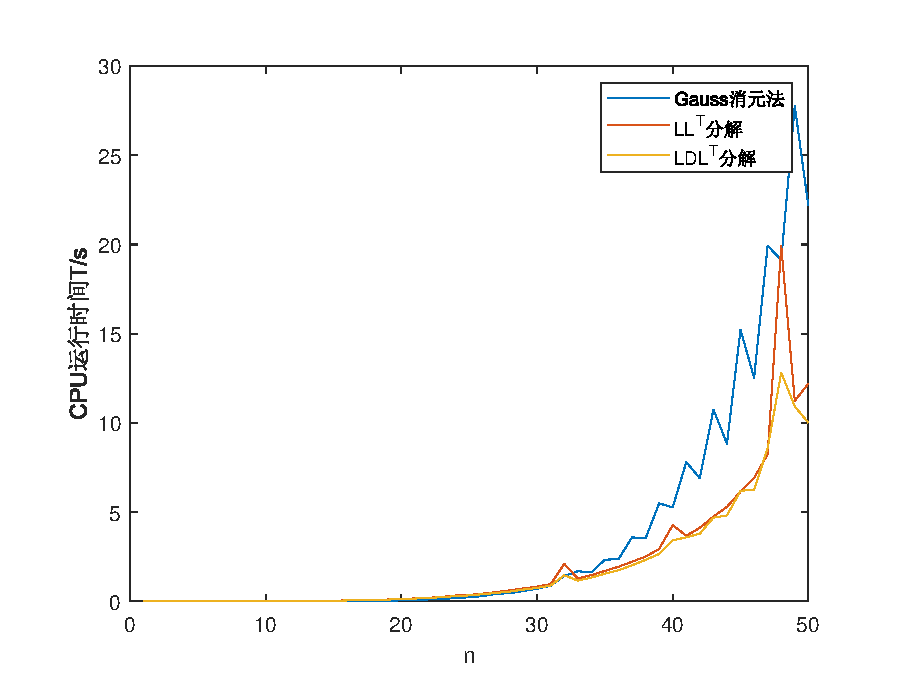
\includegraphics[width=14cm,height=10cm]{1.1_cpu_time.eps}
    \caption{The CPU running time of three direct methods}
\end{figure*}
\begin{figure*}[ht]
    \centering
    \includegraphics[width=14cm,height=10cm]{1.1_condition_number.eps}
    \caption{The condition number $\kappa_{\infty}(\mathbb{A}_{n^2})$ of the matrix $\mathbb{A}_{n^2}$}
\end{figure*}
\begin{figure*}[ht]
    \centering
    \includegraphics[width=14cm,height=10cm]{1.1_estimation.eps}
    \caption{The estimation of the constant $C$ in formula (1.4.26)}
\end{figure*}
\begin{figure*}[ht]
    \centering
    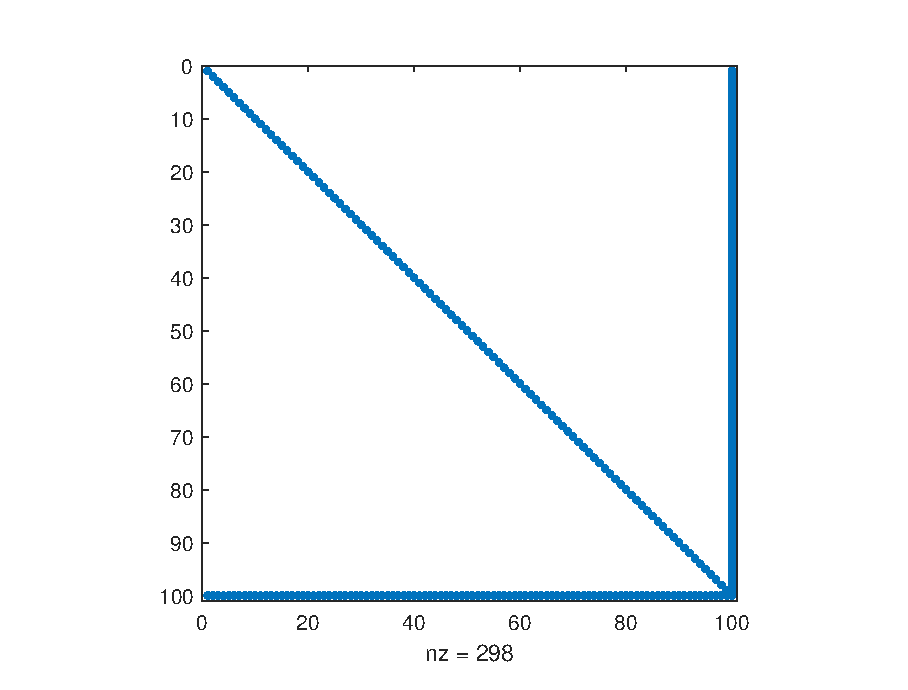
\includegraphics[width=14cm,height=10cm]{1.2_spy_B1.eps}
    \caption{The visualized sparsity pattern of matrix with the form of $\mathbb{B}_1$}
\end{figure*}
\begin{figure*}[ht]
    \centering
    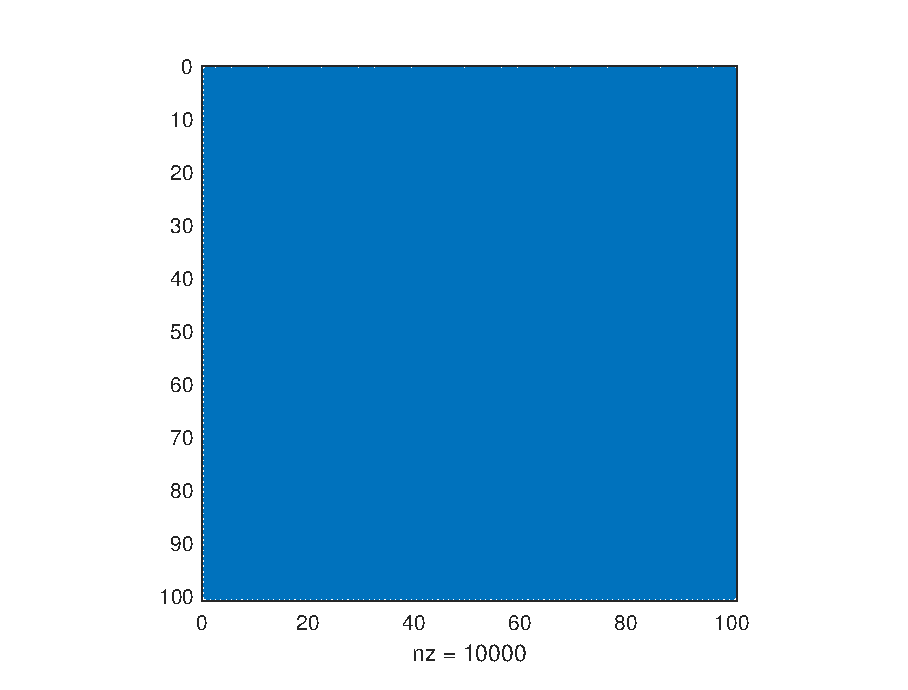
\includegraphics[width=14cm,height=10cm]{1.2_spy_B2.eps}
    \caption{The visualized sparsity pattern of matrix with the form of $\mathbb{B}_2$}
\end{figure*}
\begin{figure*}[ht]
    \centering
    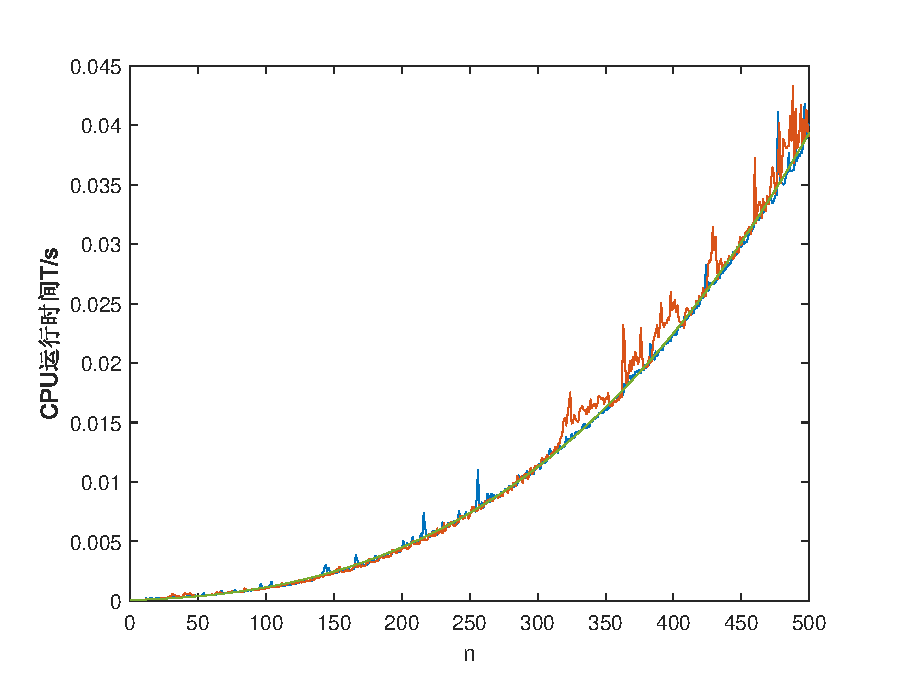
\includegraphics[width=14cm,height=10cm]{1.2_original.eps}
    \caption{The comparison of CPU running time by calculating using the original Crout algorithm}
\end{figure*}
\begin{figure*}[ht]
    \centering
    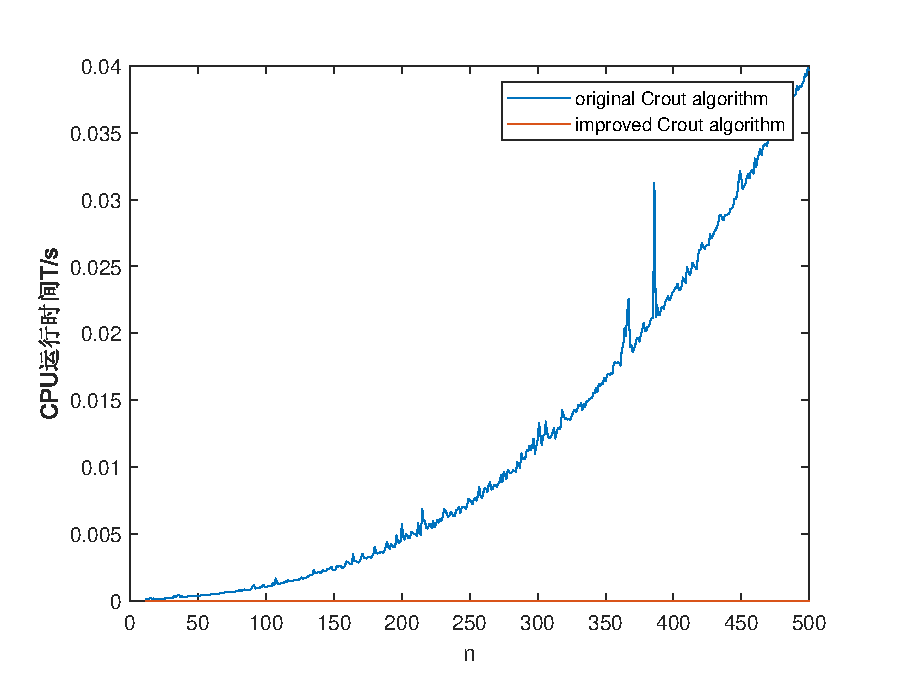
\includegraphics[width=14cm,height=10cm]{1.2_B1_comparison.eps}
    \caption{The case of $\mathbb{B}_1$ using the original and improved Crout algorithm separately}
\end{figure*}
\begin{figure*}[ht]
    \centering
    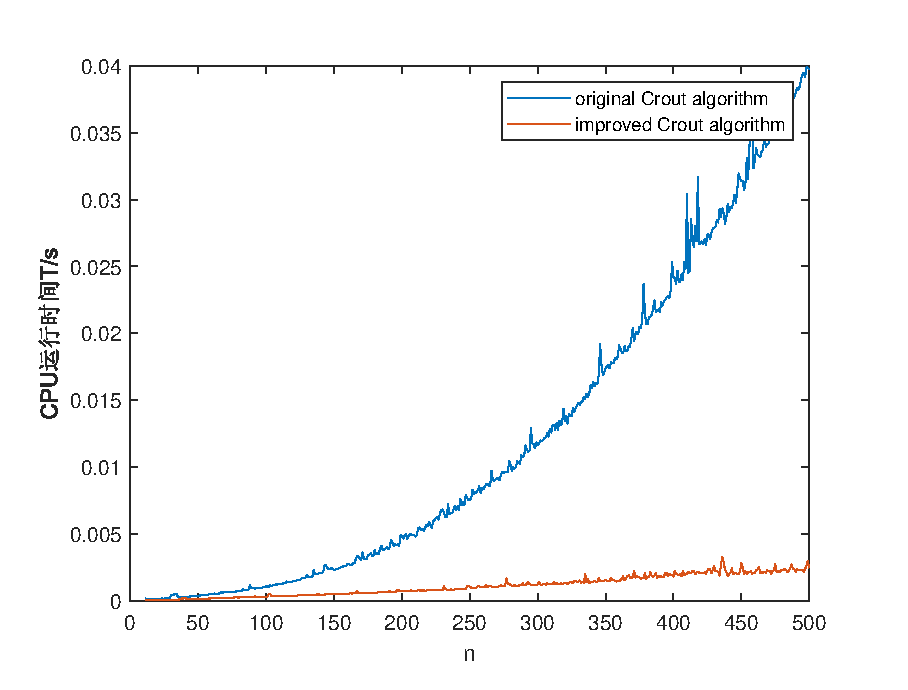
\includegraphics[width=14cm,height=10cm]{1.2_B2_comparison.eps}
    \caption{The case of $\mathbb{B}_2$ using the original and improved Crout algorithm separately}
    \end{figure*}
\begin{figure*}[ht]
    \centering
    \includegraphics[width=14cm,height=10cm]{1.3_cpu_time.eps}
    \caption{The CPU running time by calculating the inverse of $\mathbb{T}_n$}
\end{figure*}
\begin{figure*}[ht]
    \centering
    \includegraphics[width=14cm,height=10cm]{1.4_numerical_error.eps}
    \caption{The numerical error using chasing algorithm}
\end{figure*}

\section*{参考文献}
[1]林成森. 数值计算方法(上册)[M]. 北京: 科学出版社, 2005.
\end{document}
